\section{Introduction}
\label{sec:introduction}

% state the learning objective 
In this laboratory assignment we study the RC circuit 
shown in Figure~\ref{fig:circuit}. The report is divided in two main 
sections.

We started with the theoretical analysis of the circuit, 
using both nodal and mesh analysis. 
This procedure is explored in section ~\ref{sec:analysis};
We used the software \textit{Octave} to solve the derived systems 
of equations and to plot solutions.

Following this, we simulated the circuit using the software 
\textit{Ngspice}. Subsequently we compared the results of the 
simulation with the theoretical results. 
This is described in section ~\ref{sec:simulation}.

Finally, the conclusions of this study are indicated in
Section~\ref{sec:conclusion}.

\begin{figure}[ht] \centering
    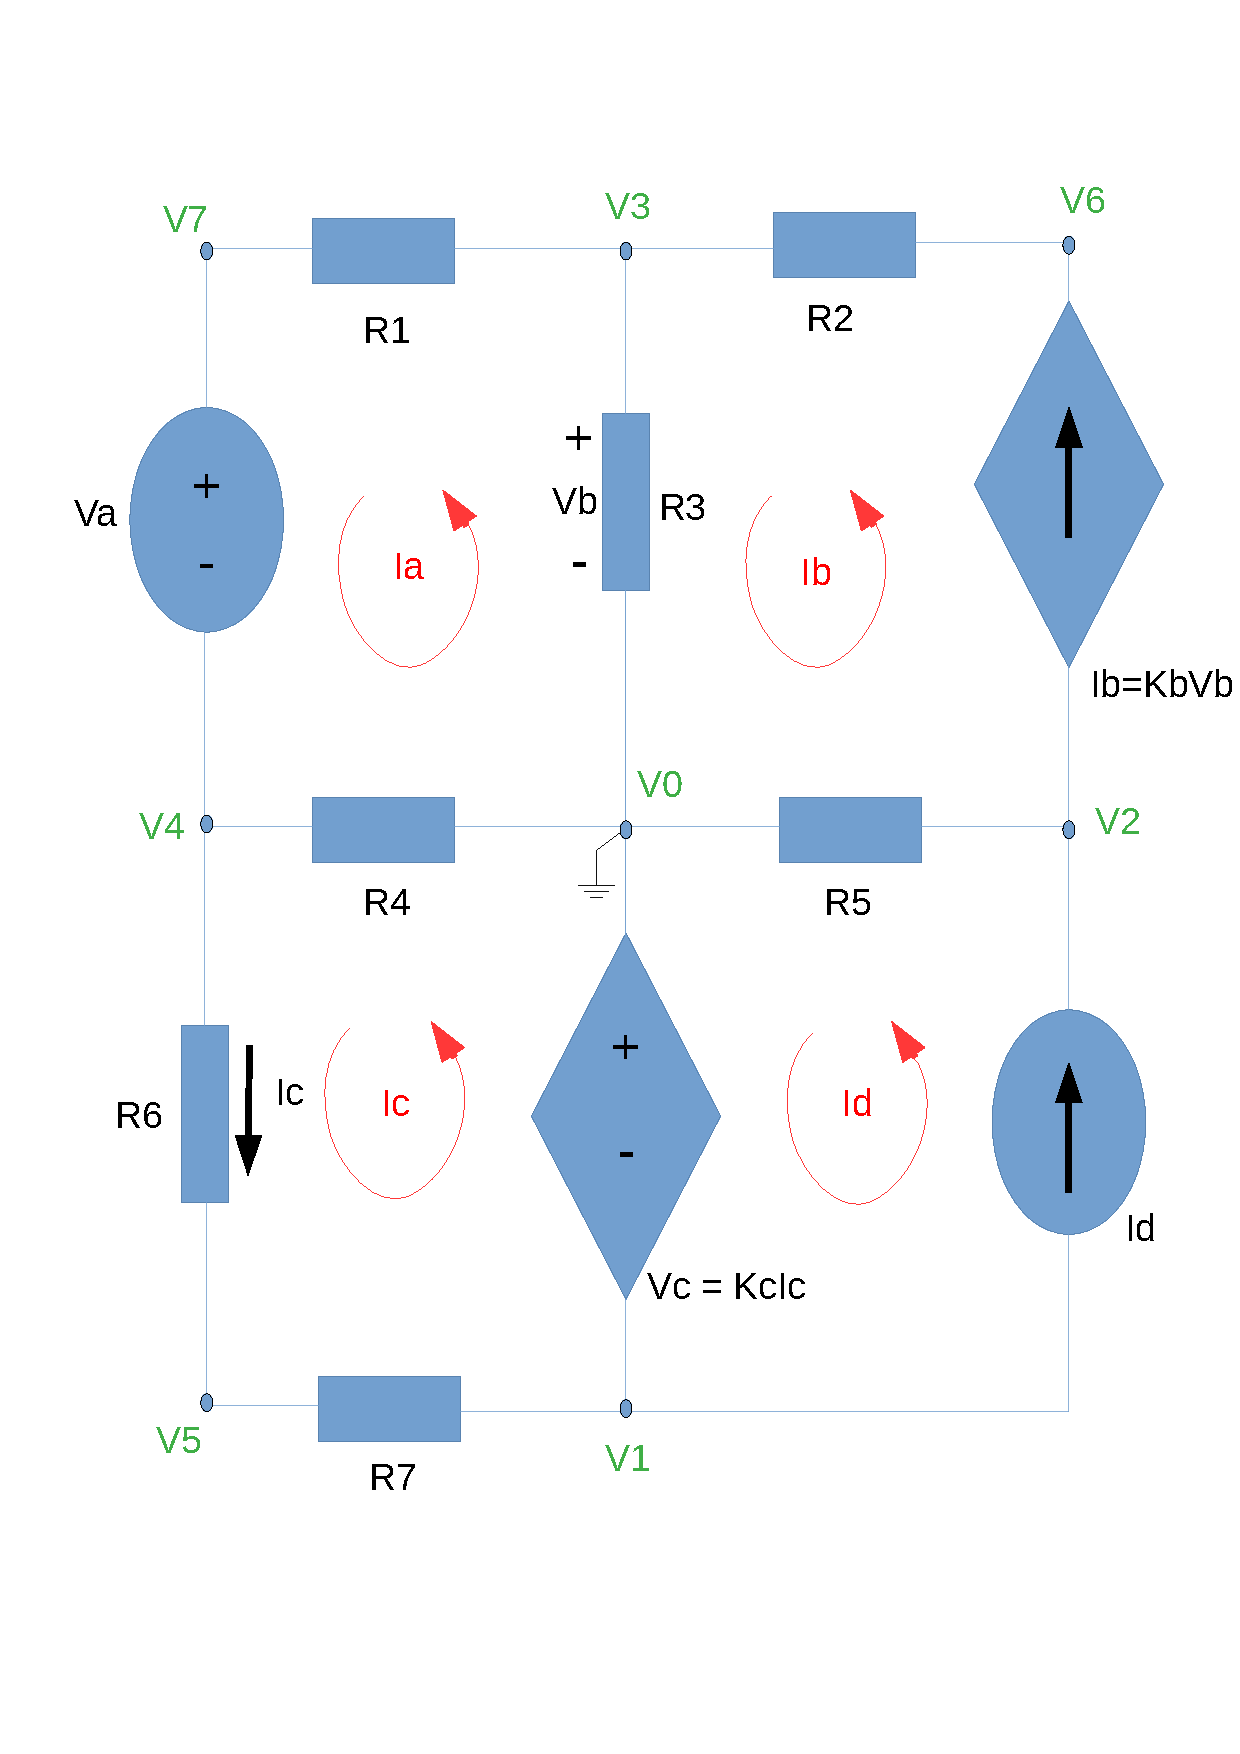
\includegraphics[width=0.4\linewidth]{circuito_tcfe.pdf}
    \caption{Circuit}
    \label{fig:circuit}
\end{figure}

